
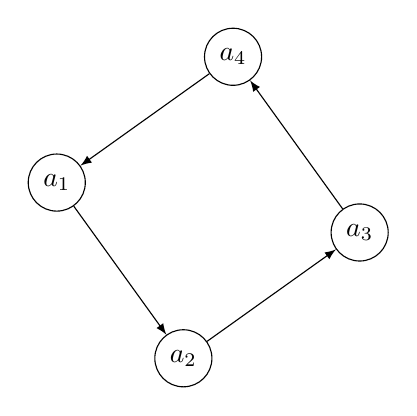
\begin{tikzpicture}[>=latex,line join=bevel,]
%%
\node (a_4) at (8.9438bp,54.271bp) [draw,circle] {$a_4$};
  \node (a_3) at (54.52bp,-8.9849bp) [draw,circle] {$a_3$};
  \node (a_2) at (-8.9438bp,-54.271bp) [draw,circle] {$a_2$};
  \node (a_1) at (-54.52bp,8.9849bp) [draw,circle] {$a_1$};
  \draw [->] (a_2) ..controls (15.637bp,-36.73bp) and (20.924bp,-32.958bp)  .. (a_3);
  \draw [->] (a_3) ..controls (36.867bp,15.515bp) and (33.071bp,20.785bp)  .. (a_4);
  \draw [->] (a_1) ..controls (-36.867bp,-15.515bp) and (-33.071bp,-20.785bp)  .. (a_2);
  \draw [->] (a_4) ..controls (-15.637bp,36.73bp) and (-20.924bp,32.958bp)  .. (a_1);
%
\end{tikzpicture}
